\subsection{Modelo Matemático de SEIR}
Debido a los problemas y suposiciones del modelo SIR, múltiples variaciones han sido creadas a lo largo del tiempo para ayudar a los científicos e investigadores a simular y estudiar mejor sistemas de epidemiología. El modelo SEIR nace como uno de estos, en donde el problema en que las personas expuestas al virus se vuelven infecciosas inmediatamente. La forma de solución, es generar un nuevo estado para una persona de la población susceptible inicial llamado 'expuesto', donde una persona ya fue infectada, pero aún no es capaz de transmitir la infección a otras de la población susceptible.

Sin embargo, este modelo clásico sigue generando un par de problemas de ambiguedad y suposiciones, por lo que, para el caso del COVID-19, investigadores procuraron modificarlo incluso más, para mejor modelar la enfermedad.

\begin{figure}
    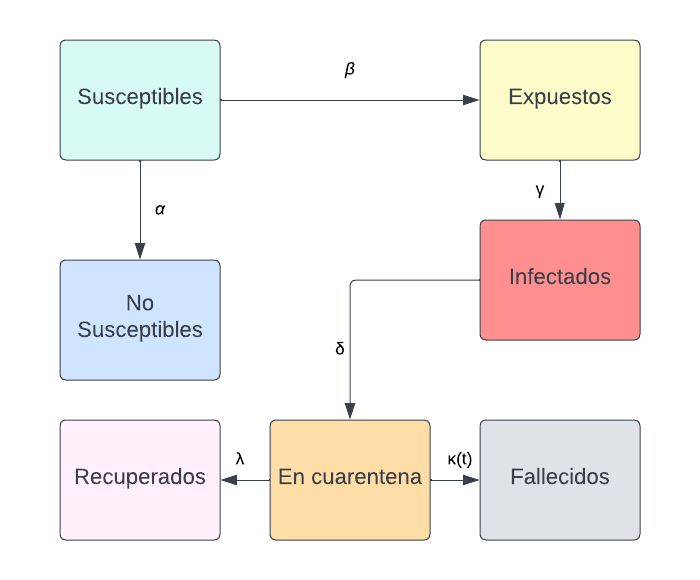
\includegraphics[width=\columnwidth]{Diagrama SEIR.png}
    \caption{Diagrama de estados de una persona en el modelo SEIR, basado en la caracterización hecha por Peng y colaboradores. Elaboración propia.}
    \label{diagrama SEIR}
\end{figure}

El modelo clásico SEIR se compone de las siguientes cuatro ecuaciones:
\begin{eqnarray}
    \frac{dS(t)}{dt} = - \beta * \frac{S(t) I(t)}{N} \label{SEIR1}\\
    \frac{dE(t)}{dt} = \beta * \frac{S(t) I(t)}{N} - \gamma E(t) \label{SEIR2}\\
    \frac{dI(t)}{dt} = \gamma E(t) - \delta I(t) \label{SEIR3}\\
    \frac{dR(t)}{dt} = \delta I(t) \label{SEIR4}
\end{eqnarray}

Este modelo de cuatro estados describe entonces, en su ecuación \eqref{SEIR1}, el cambio de población susceptible en un instante, \eqref{SEIR2}: el cambio de su población expuesta en un instante, \eqref{SEIR3}: el cambio de su población infectada en un instante, y finalmente, \eqref{SEIR4}: el cambio de su población recuperada en un instante.

Lianrong Peng, y colaboradores, describen en un documento de título "Análisis epidémico del COVID-19 en China mediante modelación dinámica"\cite{https://doi.org/10.48550/arxiv.2002.06563}, un modelo basado en el Modelo SEIR que introduce 7 estados para la población, descritos en la figura \ref{diagrama SEIR}. Este modelo modifica las ecuaciones básicas del modelo SEIR con el fin de mejor representar la epidemia a fecha de 2020. Descrito abajo se muestra los siete estados descrito por Peng y colaboradores:

\begin{equation} \label{PENG}
    \begin{split}
    \frac{dS(t)}{dt} & = - \beta * \frac{S(t) I(t)}{N} - \alpha S(t) \\
    \frac{dE(t)}{dt} & = \beta * \frac{S(t) I(t)}{N} - \gamma E(t) \\
    \frac{dI(t)}{dt} & = \gamma E(t) - \delta I(t) \\
    \frac{dQ(t)}{dt} & = \delta I(t) - \lambda(t) Q(t) - \kappa(t) Q(t) \\
    \frac{dR(t)}{dt} & = \lambda(t) Q(t) \\
    \frac{dD(t)}{dt} & = \kappa(t) Q(t) \\
    \frac{dP(t)}{dt} & = \alpha S(t)
    \end{split}
\end{equation}

En este sistema, las ecuaciones representan lo siguiente:
\begin{itemize}
    \item S(t): el número de casos susceptibles.
    \item E(t): el número de casos expuestos, aquellos que han sido infectados por el virus, pero aún no tienen la capacidad de transmitirlo ellos mismos.
    \item I(t): el número de personas que han sido infectadas, y que no han sido puestos en cuarentena.
    \item Q(t): el número de casos en cuarentena, aquellos que son positivos en la enfermedad, y son puestos en una condición que les imposibilita infectar a otros.
    \item R(t): el numero de casos recuperados o curados.
    \item D(t): el número de casos que han fallecido.
    \item P(t): el número de casos no susceptibles. Son aquellos que se han protegido o inmunizado, y ya no contraen la enfermedad.
\end{itemize}

De forma similar a como se hizo para el modelo SIR, se puede obtener la siguiente expresión, donde N es nuevamente la población inicial cerrada:

\begin{equation}
    S + E + I + R + Q + R + D + P = N
\end{equation}

